\begin{WyrdScenarioHeading}[The Clockmaker's Deception]{The Clockmaker's\\ Deception}
    \label{scenario:clockmakers-deception}
    \index{The Clockmaker's Deception}
    \index{The Clockmaker's Deception!Scenario}

    A shocking murder has thrown London’s scientific and industrial circles into disarray. The esteemed inventor, \textbf{Dr Sebastian Thorne}, stands accused of killing a rival engineer, \textbf{Arthur Bellamy}, who was found dead in Thorne’s workshop. The evidence against him seems irrefutable—Bellamy’s body was discovered with blunt force trauma, and the only witness claims that one of Thorne’s own clockwork creations struck the fatal blow.

    But something about the case doesn’t add up. The mechanical automaton, a prototype designed to assist in fine-detail engineering, should be incapable of such an act. Was this an unfortunate accident, or has someone manipulated the scene to frame Thorne? The investigators must untangle the mystery before the city condemns a man who may be innocent—or worse, before a hidden truth shakes the foundations of science itself.

    \subsection*{Premise} 
    A renowned inventor is accused of murder when his latest clockwork creation is found standing over a dead body. The case seems open and shut, but a deeper conspiracy lurks beneath the surface. Was the machine truly responsible, or is someone using technology as a convenient scapegoat?

    \subsection*{What Really Happened} 
    Arthur Bellamy had uncovered a secret — one that threatened powerful interests within London’s scientific community. He arranged a meeting with Thorne under the guise of a professional discussion, intending to share his findings. However, before he could reveal the full truth, an unknown party silenced him.

    The real killer staged the scene, positioning Thorne’s automaton as the culprit. By tampering with the machine’s mechanisms and manipulating witnesses, they ensured that suspicion would fall on Thorne. Now, as the city rushes to condemn him, the investigators must uncover the true murderer, reveal the secret Bellamy died for, and navigate the dangerous underworld of industrial espionage.
\end{WyrdScenarioHeading}

As with the previous scenario, you can act out the summoning to \textbf{The Grand Society of Inquiry} as a way to introduce the investigators to the case. If the set of player characters in this scenario differs from the player characters in the previous one, this would give you an excellent way of introducing the new characters to the players.


\begin{GmTips}
    This case provides an excellent opportunity to explore themes of scientific advancement, ethical dilemmas, and the fear of technology gone rogue. The case may also lead into larger conspiracies within London's industrial elite, depending on how deep the investigators choose to dig.
\end{GmTips}



\subsection{Act 1: The Accusation}  
The investigators are summoned to the scene of the crime—the locked workshop of Dr Thorne. The city’s authorities have already decided his guilt, but the inconsistencies in the case suggest a deeper truth. With the evidence stacked against Thorne, the investigators must uncover what really happened in the workshop that night.

\subsubsection*{The Exterior of Thorne's Laboratory}
Dr Thorne’s laboratory sits at the end of a narrow, soot-streaked lane in the Iron Quarter—London’s industrial heart, where smoke stacks and clock towers pierce the grey skyline. A black-iron gate surrounds the courtyard, normally closed to the public, but today it's flung wide. Two constables stand guard at the entrance, keeping a tense eye on the small but growing crowd gathered just beyond the perimeter.

A group of protestors—members of the \textbf{Aetheric Liberty Assembly}—have assembled outside. Their banners bear slogans like \textbf{“Gears Deserve Guidance”} and \textbf{“Stop Mechanical Murder”}. Though peaceful for now, their chants are loud, angry, and unsettling. The investigators must push through this cacophony of metal and morality to reach the crime scene.

The building itself is a multi-storey brick structure reinforced with iron beams. Pipes twist along its surface like veins, venting steam and chemical heat into the morning air. Mechanical pigeons roost on copper eaves. Through narrow windows, dim light flickers—some from gas lamps, others from arcane equipment humming behind frosted glass.

The front door bears the sigil of Thorne’s personal mark: a gear encircling a flame. It hangs slightly ajar. A Scotland Yard constable is guarding the door, instructed to let the investigators in.

\subsubsection*{The Interior of Thorne's Laboratory}

Inside the workshop, Inspector Quentin Hale (page \pageref{npc:inspector-hale}) oversees the crime scene. Though clearly displeased by the investigators’ presence, he has been overruled—political pressure has placed the Grand Society in charge. Hale may grumble, but he will not obstruct their work.

The workshop is dimly lit, the air tinged with oil, ozone, and burnt brass. Workbenches stretch along both walls, cluttered with delicate tools, sketched blueprints, and parts of half-assembled inventions. A network of copper pipes and reinforced cables snake along the ceiling, feeding power to humming dynamos and mechanical arms suspended like skeletal limbs above the tables.

The heart of the room is dominated by a large brass automaton—Thorne’s prototype—standing still beside the body of \textbf{Arthur Bellamy}. The automaton’s plating is burnished and elegant, its hands designed for fine manipulation. One arm is slightly raised, locked in a half-motion that could suggest violence—or simply an aborted action.

Several clues are immediately apparent to trained eyes:

\begin{itemize}\raggedright
    \item \textbf{Bellamy’s Body:} The victim lies sprawled on the tiled floor. His head is crushed, consistent with blunt force trauma. However, \textbf{Investigate} \DL{+1} will reveal that there are no defensive wounds or signs of a struggle.
    
    \item \textbf{The Automaton’s Damage:} Close inspection (\textbf{Craft} \DL{+1} or \textbf{Investigate} \DL{+2}) reveals microfractures near the shoulder joints—indicative of tampering or forced override. The central control valve has been manually disengaged, and traces of a foreign compound (a dark, viscous lubricant) coat the actuators. %% FIXME: What is the foreign compound?

    \item \textbf{Disturbed Blueprints:} A nearby workbench has been recently rifled through. Among the scattered pages, one appears to be missing. The remaining documents reference a “neurological feedback loop,” an advanced theory Thorne had not yet published.

    \item \textbf{Footprints and Oil Trail:} A \textbf{Notice} \DL{+1} will reveal a thin line of the same dark lubricant leads away from the automaton and out toward a service hatch in the back wall. There are faint muddy footprints nearby—too small to be Thorne’s boots.

    \item \textbf{The Command Console:} A brass-and-glass terminal rests against the far wall, its dials flickering erratically. \textbf{Investigate} \DL{+1} reveals that the command log shows routine diagnostic entries—until the night before, when it was wiped entirely between the hours of 1:00 and 2:00 a.m.

    \item \textbf{Thorne’s Private Notes:} Hidden beneath a false panel in his desk drawer (\textbf{Notice} \DL{+3} or \textbf{Investigate} \DL{+2}), investigators may discover a leather-bound notebook. It contains sketches and ramblings about a cognition module designed to give automata limited adaptive learning—an innovation that would be highly controversial if revealed.
    
    \item If the players search Thorne’s workshop carefully (\textbf{Investigate} \DL{+2}), they may find a hidden compartment in the desk containing \textbf{a letter from Bellamy, warning Thorne of a potential betrayal}.
\end{itemize}

The foreign compound is \textbf{aetherite-infused oil}, a rare lubricant used in high-end automata. It is known to cause erratic behavior in machines when improperly applied, and its presence here suggests deliberate tampering. To discover this, the players must succedd on a \textbf{Craft} \DL{+2} or use their contacts to get the substance examined in a laboratory.

\subsubsection*{Witnesses and Testimonies}
Once inside the laboratory, the investigators will have the opportunity to speak with the key witnesses remaining on site. Each has a different perspective on the events of the night in question, though their accounts are not without inconsistencies. How much they reveal—and whether they can be trusted—is for the players to determine.

\vspace{\baselineskip}
\paragraph{Dr Sebastian Thorne}
A gaunt, intense man in his late fifties, Thorne paces restlessly, his cuffs soot-stained and his eyes ringed with exhaustion. He insists on his innocence, though his account is fragmented and at times erratic.

\begin{itemize}
    \item Thorne claims that Bellamy came to visit late in the evening, requesting a private meeting to discuss a “matter of great urgency.” He led Bellamy into the workshop and briefly left him alone to retrieve a notebook from his upper study.
    \item When Thorne returned—less than ten minutes later—he found Bellamy dead and the automaton standing motionless beside the body.
    \item He insists that the automaton lacks any capacity for violent action and was in standby mode at the time.
    \item Under pressure, Thorne may admit he was working on a cognition module that would allow the machine to adapt to user needs, but he has not installed it yet.
\end{itemize}

Thorne is defensive, paranoid, and deeply shaken. He’s also terrified of what will happen if his work falls into the wrong hands. A successful \textbf{Empathy} \DL{+1} check may reassure him enough to reveal more about his experimental designs or recent disagreements with Bellamy.



\begin{CommentBox}{Thorne and Bellamy’s Disagreement}  
    The two men were once colleagues, working together on the early principles of adaptive automata—machines capable of limited aetheric cognition. Their paths diverged when Bellamy became alarmed by the implications of their work. He feared that sentient machines could become unstable or be exploited by unscrupulous industrial forces. Thorne, on the other hand, argued for the careful and ethical application of these technologies, believing in their transformative potential.
    
    Six months prior to the murder, Bellamy publicly denounced Thorne’s research at a symposium, calling it “reckless” and “morally blind.” The rift became personal and professional. Since then, Thorne had grown reclusive, while Bellamy pursued independent inquiries—some of which may have uncovered secrets worth killing for.
    
    \textbf{FIXME:} This history gives context to their final meeting. Bellamy may have come to offer a warning, a truce, or a final accusation. Whatever the intent, it placed him in the automaton’s shadow for the last time.
\end{CommentBox}


\vspace{\baselineskip}
\paragraph{Neville Crowsley, Workshop Assistant}
A factory labourer in his twenties, Crowsley claims to have seen the automaton kill Bellamy. He is currently being held under police supervision in the neighbouring antechamber.

\begin{itemize}
    \item Crowsley says he entered the workshop in response to a strange noise and saw the automaton lurch forward, striking Bellamy down.
    \item However, his account is vague on specifics—he can’t describe where Thorne was at the time, and he avoids direct eye contact when questioned.
    \item \textbf{Empathy} \DL{+2} or \textbf{Provoke} \DL{+1} may reveal signs of anxiety and hesitation. He may be hiding something or repeating a rehearsed version of events.
    \item A successful \textbf{Investigate} \DL{+2} of Crowsley’s effects might uncover a recent payment stub from a company linked to one of Thorne’s industrial rivals.
\end{itemize}

Crowsley is not a malicious man, but he may have been bribed, intimidated, or simply afraid of losing his job. The investigators must decide whether to press him or win his trust.

\begin{CommentBox}{The Truth Behind Crowsley’s Account}
    Crowsley was in the workshop when Bellamy arrived, but he was not present when the automaton struck. He heard the commotion and rushed in to find Bellamy dead. The automaton was still standing, but it had not moved. Crowsley panicked and fled, but someone caught him outside and offered him a bribe to testify against Thorne.
\end{CommentBox}


\subsubsection*{What Actually Happened}
While Dr Thorne was away from the workshop for approximately ten minutes, the real killer—already hiding inside the building—acted swiftly and with purpose.

\paragraph{The Murder:}
Arthur Bellamy had come to confront Thorne with a warning: he believed someone was misusing or stealing advances in aetheric cognition. He suspected Thorne’s research had been compromised, though he may not have known by whom. While waiting alone in the workshop, Bellamy reviewed one of the prototype’s exposed schematics—unaware that he was being watched.

The killer struck from behind with a heavy gear calibration tool, delivering a single fatal blow to the back of Bellamy’s skull. The murder weapon was hastily wiped and thrown into a disposal chute connected to the lower furnace. The body was left beside the automaton in a carefully posed sprawl.

\paragraph{The Tampering:}
To stage the scene, the killer sabotaged the automaton:
\begin{itemize}
    \item \textbf{Override Control:} Using a smuggled mechanical override key, they manually disengaged the automaton’s central valve and rewrote part of its posture routine, forcing its arm into a half-raised state—as if mid-swing.
    
    \item \textbf{Aetherite-Infused Oil:} The saboteur applied a thin layer of \textbf{aetherite-infused lubricant} to key actuator joints. This compound, known to cause unstable behaviour in uncalibrated automata, would imply erratic motion to the untrained eye.
    
    \item \textbf{Console Tampering:} The command terminal was accessed and its logbook wiped between 1:00 and 2:00 a.m.—the estimated time of death. Only someone with technical knowledge and physical access could have executed the erasure.
\end{itemize}

By the time Thorne returned, the killer was gone—vanished through the rear service hatch, leaving only a trail of oil and carefully manipulated suspicion in their wake.



\subsection{Act 2: Through Brass and Smoke}
As the investigation deepens, it becomes clear that Bellamy’s death was no accident. The crime was carefully staged to look like mechanical failure—but the sabotage runs deeper. Several scenes are now available for investigation, each revealing a different facet of the emerging conspiracy.

\subsubsection{The Aetheric Liberty Assembly}
\textbf{Dr Octavius Wren} (page~\pageref{npc:octavius-wren}), leader of the Aetheric Liberty Assembly, arrives demanding to speak with the investigators. Passionate and unyielding, Wren believes powerful industrialists are experimenting with automata and aetheric control systems to build soldiers that obey without question—and that Bellamy’s death was an execution, not an accident.

While Wren cannot offer proof, his words may plant doubt. He suggests that Evelyn Baker or another rival inventor may be involved, and warns the investigators that if the truth isn’t exposed, more “accidents” will follow.

\subsubsection*{The Chemical Analysis}

If the players arrange for a lab to analyse the foreign lubricant, results return within hours via Society courier or trusted contact.

\begin{itemize}\raggedright
  \item \textbf{Composition:} The oil is aetherite-infused and reactive under high-frequency pulses. It is not commercially available and its synthesis will leave a unique trace to the lab where it was produced.
  \item \textbf{Supplier Lead:} A trace additive points to a batch produced by \textbf{Gideon \& Sons Mechanical Works}, a firm with ties to Thorne’s industrial rivals, \emph{Greymark Aetherworks Ltd}.
  \item \textbf{Cover-Up Attempt:} Records show someone recently altered the facility’s shipment logs—suggesting an attempt to conceal the oil’s origin.
\end{itemize}

This clue links the tampering to a well-resourced organisation and provides leverage to confront those with access to rare materials.


\subsubsection{Word on the Street}
If the players seek information in the Iron Quarter’s alleys and underbelly, local informant \textbf{Kip “Knuckles” Mallory} (page~\pageref{npc:kip-mallory}) proves useful. Over a tin mug of gin or a clinking bribe, he shares a name: \textbf{Evelyn Baker}, a ruthless inventor known for industrial espionage.

A player using \textbf{Contacts} may discover Evelyn’s name through other channels:
\begin{itemize}
    \item \DL{+1} if asking specifically about Bellamy’s associates or suspected espionage
    \item \DL{+2} for a general search across London’s inventor and patenting circles
\end{itemize}

Baker was recently seen near Thorne’s lab. She has a reputation for crossing moral lines in pursuit of technological advancement—and she may have been watching Thorne for weeks.

\subsubsection*{Evelyn Baker’s Workshop}

Evelyn maintains a cluttered, well-guarded workshop in the shadow of a disused tram station. The front is locked with a reinforced cipher lock (\textbf{Burglery} \DL{+2} to pick, or \textbf{Contacts} \DL{+1} to obtain a stolen passcode). Inside, players may uncover:

\begin{itemize}
  \item \textbf{Bellamy’s Schematic Fragment:} A torn blueprint page bearing Bellamy’s initials—part of the same set missing from Thorne’s lab.
  \item \textbf{Aetherite Samples:} Locked in a supply drawer are two vials of \textbf{aetherite-infused oil}, identical to the compound used on Thorne’s automaton.
  \item \textbf{Sabotage Contracts:} A coded ledger (decrypt with \textbf{Lore} \DL{+2}) containing a contract referring to the “controlled discrediting of autonomous systems.”
\end{itemize}

If confronted, Evelyn denies the murder but admits she was hired to apply pressure on Thorne. She insists Bellamy’s death was not part of her assignment. She can, however, intimidated or bribed into revealing the client that hired her to spy on Thorne: \textbf{Lord Ashford Greymark}.

\subsubsection*{Lord Ashford Greymark}

The true architect behind Bellamy’s death is \textbf{Lord Ashford Greymark}, a peer of the realm with deep ties to the Ministry of Defence. Greymark holds a long-standing contract to produce military-grade automata for deployment in colonial outposts and urban policing—but despite vast funding and political support, his designs have consistently failed to meet the Ministry’s expectations.

Desperate to retain his influence and reputation, Greymark turned to espionage. Through intermediaries, he hired Evelyn Baker to spy on Dr Thorne, whose breakthroughs in cognitive stability could make military automata viable. When Bellamy—once a research associate of Greymark—discovered the scheme and threatened to expose it, Greymark acted swiftly.

When Lord Greymark learned that Bellamy was about to reveal the truth to Dr Thorne, he needed to act. He was spying on their meeting, waiting for his opportunity, and when Bellamy was alone in the workshop, he struck. 

\textbf{Exposing Greymark} requires more than proof of motive—it demands uncovering his ties to Baker, tracking the flow of stolen materials, or intercepting confidential Ministry communications. Bringing him down could shake the foundations of government oversight—and earn the investigators powerful enemies.


\vspace{\baselineskip}\noindent
By the end of Act 2, the investigators should have a suspect—but proving their guilt will require uncovering their true motive.

\WyrdFooterImage{img/pageart/gears-bottom-right-cropped}

\import{./}{npcs}


\subsection{Act 3: Beyond Reasonable Doubt}
With the clues pointing toward Lord Ashford Greymark, the investigators now face their greatest challenge: proving the truth in the face of power. Greymark’s influence shields him from direct accusation, and any misstep could see Thorne condemned and the conspiracy buried. The investigators must secure undeniable proof and decide how—and to whom—they will reveal it.

\subsubsection*{Paths to Justice}
There is no single route to exposing Greymark. Instead, players must choose how best to assemble and present the evidence:

\begin{itemize}
    \item \textbf{Trace the Sabotage Materials:} A successful infiltration or audit of Gideon \& Sons may uncover records linking shipments of aetherite-infused oil to Greymark’s Ministry project at \emph{Greymark Aetherworks Ltd}. (\textbf{Burglery} or \textbf{Contacts} \DL{+2})
    
    \item \textbf{Secure a Confession from Evelyn Baker:} With sufficient leverage—empathy, intimidation, or a deal—Baker may admit to the authorities that Greymark paid her to spy on Thorne and sow discrediting evidence. (\textbf{Empathy}, \textbf{Will}, or \textbf{Deception} \DL{+1–2})

    \item \textbf{Intercept Confidential Correspondence:} If the players infiltrate a government mail hub, bribe a clerk, or intercept a pneumatic message, they may find incriminating letters between Greymark and Ministry officials discussing “Project Compliance.” (\textbf{Investigation}, \textbf{Burglary} or \textbf{Lore} \DL{+2})
\end{itemize}

\subsubsection*{Final Confrontation}
If the players choose to confront Greymark directly—at his estate, in Parliament, or during a Ministry symposium—he will deny all charges, mock their evidence, and attempt to discredit them. Unless they have an ironclad case, the confrontation may backfire.

\begin{itemize}
    \item With enough pressure, Greymark may offer a private settlement or threaten their careers.
    \item Alternatively, he may attempt to flee, destroy evidence, or even arrange for their disappearance.
    \item If brought before a tribunal of the Grand Society or sympathetic members of the Crown, the players may use their gathered evidence to deliver a public reckoning.
\end{itemize}

\newcolumn
\subsubsection*{Possible Outcomes}

\begin{itemize}
    \item \textbf{Greymark is Exposed:} The evidence is overwhelming. Greymark is stripped of his contracts, his estate raided, and Thorne exonerated. The Grand Society earns respect—but also powerful enemies.
    
    \item \textbf{Justice, at a Cost:} Greymark is forced to resign quietly. Thorne is cleared, but the truth is suppressed to avoid scandal. The players are warned to stop digging—permanently.
    
    \item \textbf{The Truth Is Buried:} The players fail to produce sufficient proof. Thorne faces sentencing, and Greymark’s plans move forward. Only the investigators know the truth—and their time will come.
\end{itemize}

However the act ends, the investigators leave changed—and the gears of conspiracy keep turning in the shadows of London.

\vspace*{\fill}
\begin{center}
    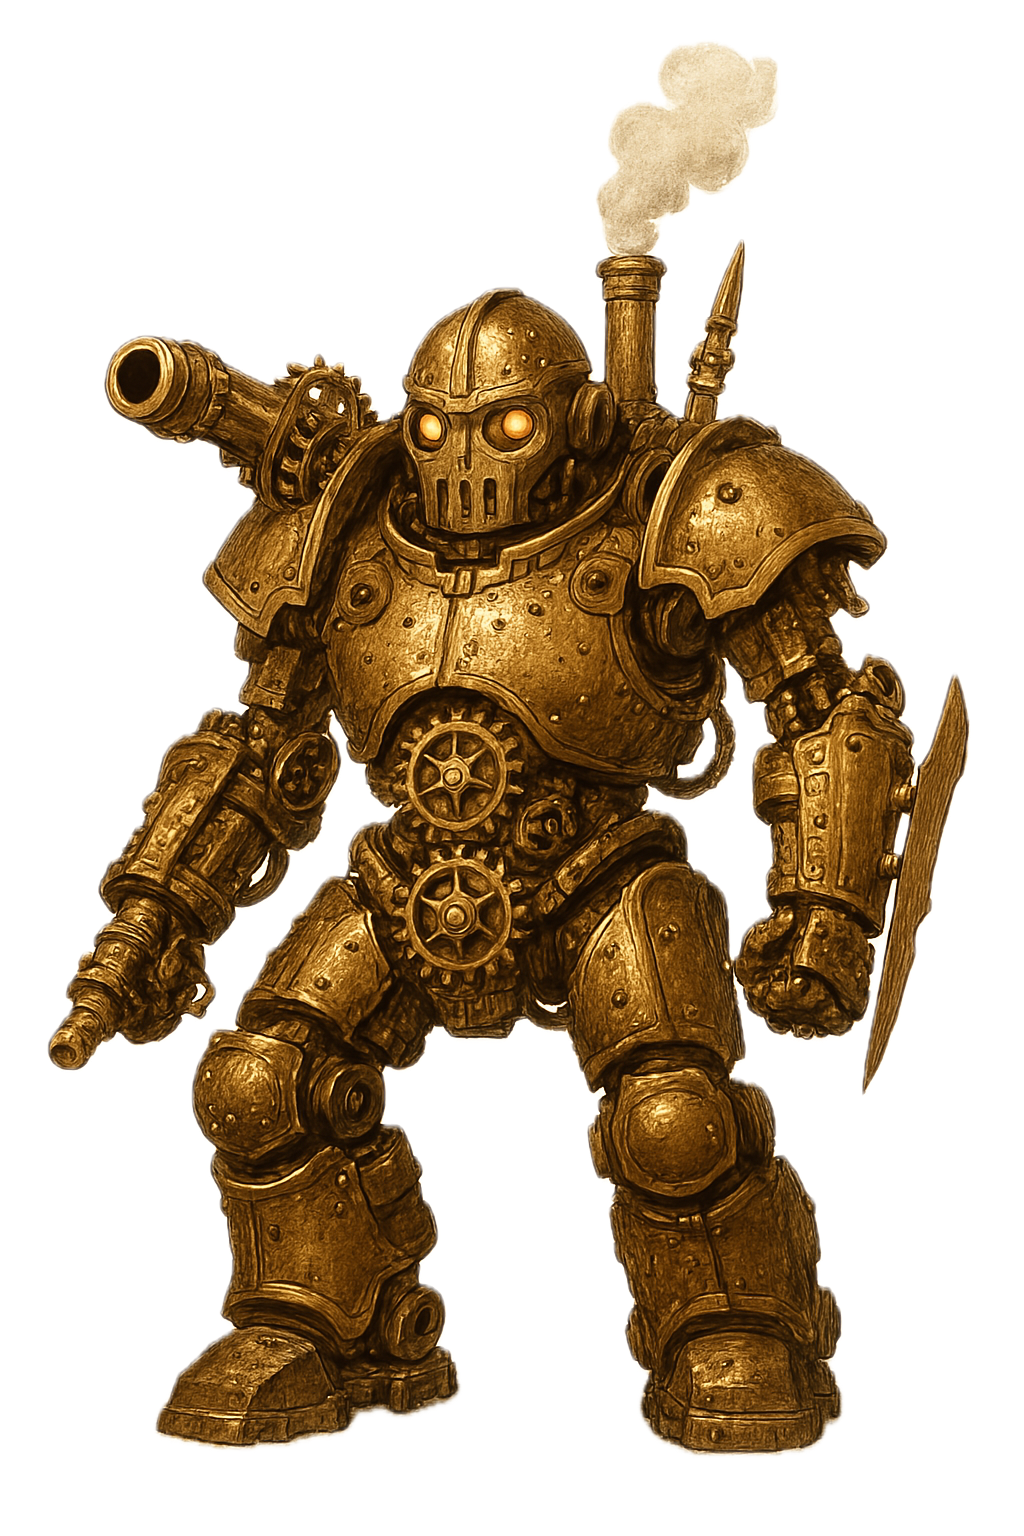
\includegraphics[width=\linewidth]{img/separt/army-automaton}
\end{center}
\vspace*{\fill}


%% Hack for formatting columns before the next scenario
\end{multicols}
\newpage
\begin{multicols}{2}
